\chapter{Pose Estimation}\label{ch:2-pose-estimation}

This chapter focuses on pose estimation, specifically addressing the optimization-based PCR problem. It introduces the \gls{rcqp} and \gls{gnc} methods used to solve this problem and evaluates their performance in estimating the pose of the object of interest. The primary objective is to assess the extent to which \gls{rcqp} and \gls{gnc} can accurately estimate the position and orientation of the object, aiming for a \SI{95}{\percent} accuracy level as mentioned in \secref{sec:intro-problem-description}. Importantly, it is assumed throughout the chapter that the object of interest is known, eliminating the need for classification.\medskip

To achieve this goal, the chapter presents the methodologies employed, the experimental setup, and the obtained results. The results obtained in this chapter encompass two main aspects 1) synthetic source data is utilized, and generated from the target data to ensure accurate correspondences. This allows for the evaluation of the methods' robustness by introducing varying percentages of outliers. 2) the methods are applied to sampled data from~\chapref{ch:1-tactile-perception} to estimate the pose of the object based on computed correspondences.\medskip

Furthermore, in addition to solving the pose estimation problem, the chapter includes an estimation of the signal-to-outlier ratio. This is achieved by utilizing the weights produced by \gls{gnc}. The estimation is conducted firstly on the synthetic source data where the ground truth is known and secondly on the sampled source data where the outlier ratio is unknown.

% In this chapter, the pose estimation is presented as an optimization-based \gls{pcr} problem, along with the \gls{rcqp} and \gls{gnc} methods used for solving said problem and their performance in solving the \gls{pcr} problem. The goal of this chapter is to determine to what extent \gls{rcqp} and \gls{gnc} are capable of sufficiently estimating the pose of the object of interest. According to~\ref*{sec:intro-problem-description} \SI{95}{\percent} accuracy in both position and orientation estimates. It is throughout this chapter assumed that the object of interest is known, and thus no classification is needed. \medskip

% This is achieved by presenting the methods used, along with the experimental setup and results. The results gained in this chapter will be two fold 1) The methods will be performed on synthetic source data, meaning point clouds generated from the target data to ensure accurate correspondences while enabling the enforcement of certain outliers percentages, which will be applied to determine the methods robustness. 2) the methods will be applied on sampled data from~\chapref{ch:1-tactile-perception} to determine the object's pose from computed correspondences. \medskip

% In addition to the pose estimation problem solved, the signal-to-outlier ratio is estimated based on the weights produced by \gls{gnc}, first on the synthetic source data where the \gls{gt} in known and secondly on the sampled source data where the outlier ratio is unknown. \medskip

\section{Problem}\label{sec:2-pose-estimation-problem}



In this chapter, the \gls{rcqp} method with \gls{gnc} will be presented along with its performance in solving the \gls{pcr} problem. The produced source data \mat{X} in~\chapref{ch:1-tactile-perception} is a \gls{pc} of the form
%
\begin{equation} \label{eq:data-matrix-structure}
	\mat{X} = 
	\begin{bmatrix}
		c_x & c_y & c_z & n_x & n_y & n_z \\
		c_x & c_y & c_z & n_x & n_y & n_z \\
		 &  & \vdots &  &  &  \\
		c_x & c_y & c_z & n_x & n_y & n_z \\
	\end{bmatrix}\inR{M\times 6},
\end{equation}

where \mvar{\vec{c}=\rvec{c_x, c_y, c_z}} is a contact point, \mvar{\vec{n}=\rvec{n_x, n_y, n_z}} is the corresponding point's normal vector and \mvar{M} is the number of source data points. The target data \mat{Y} is structured likewise, except for the number of target data points being \mvar{N}, where \mvar{N\ge M}. For convenience, the \mvar{i}'th row in source data is referred to as \mvar{\vec{x}_i} while the \mvar{i}'th row in the target data is referred to as \mvar{\vec{y}_i}. \medskip 

Under the assumption of already knowing the object of interest, \mat{Y} is generated from the mesh of the Stanford bunny model~\cite{stanford-bunny} with a resolution of \num{10,000} data points as shown in figure~\figref{fig:pe-pc-target}. The source data \mat{X} can likewise be seen in~\figref{fig:pe-pc-source} as generated in~\chapref{ch:1-tactile-perception}. \medskip

\begin{figure}[!h]
	\centering
	\begin{subfigure}[b]{0.48\textwidth}
		\centering
		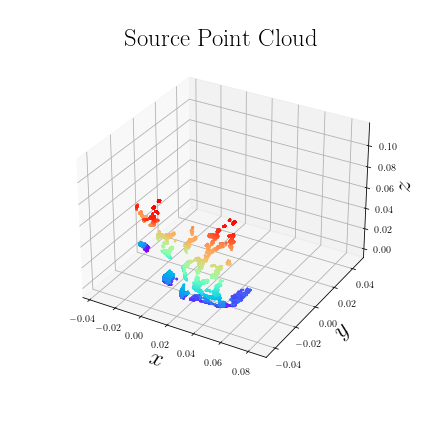
\includegraphics[width=\textwidth]{chapters/1-tactile-perception/fig/matplotlib/pc_source.png}
		\caption{The source data \mat{X} \gls{pc} generated from simulated contact points, normals are also included, but not illustrated here for the sake of simplicity.}
		\label{fig:pe-pc-source}
	\end{subfigure}
	% \hfill
	\begin{subfigure}[b]{0.48\textwidth}
		\centering
		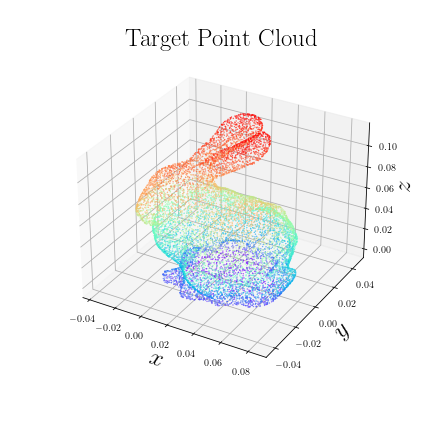
\includegraphics[width=\textwidth]{chapters/1-tactile-perception/fig/matplotlib/pc_target.png}
		\caption{The target \gls{pc} generated by sampling the model mesh with \num{10,000} points, normals are also included, but not illustrated here for the sake of simplicity.}
		\label{fig:pe-pc-target}
	\end{subfigure}
	\caption{3D plots showing source and target data.}
	\label{fig:pe-contact-position-gazebo}
\end{figure}

To determine the transformation between the two point clouds \tf[T]{\mat{X}}{\mat{Y}}, correspondences must be found according to the \gls{corr-problem}. Due to \mat{X} being produced by local sensing with high-density sensor regions, a \gls{pc} feature which exploits this is desired. The one chosen is \gls{fpfh} which is a feature descriptor used in 3D point cloud analysis and registration tasks and provides a feature matrix \mvar{\mat{F}\inR{N\times 33}}. The feature descriptor calculates a histogram representation for each point by considering the local geometric properties of its neighboring points. It captures information about the distribution of surface normals and distances between points within a local neighborhood. Additionally, \gls{fpfh} is computationally efficient and provides robust feature representations. \medskip

Using the correspondences found from \gls{fpfh}, the pose estimation problem can be formulated as an optimization problem for determining the optimal homogeneous transformation matrix between the two points clouds \tf[T]{\star\mat{X}}{\;\;\mat{Y}}, which for convenience is from now on referred to as \tf[T]{\star}{}, by
% \colorbox{red}{obs, what makes GNC special is the fact that it changes the \mvar{\mu} either up or down depending on GM or TLS, which gradually causes non-convexity. RCQP is used to solve for x in gnc paper}
%
\begin{equation} \label{eq:point-cloud-registration-problem}
	\tf[T]{\star}{} = \arg \min_{(\mat{R},\vec{t})\in\SE (3)} \sum^M_{i=1} d_{P_i}\left( \mat{T} \oplus \vec{x}_i \right)^{2}.
\end{equation}

Here \mvar{\tf[T]{}{}=(\tf[R]{}{}, \vec{t})\in\SE (3)} refers to the homogeneous transformation matrix \mvar{\tf[T]{}{}\inR{4\times 4}} from \mat{X} to \mat{Y}, which consists of a rotation matrix \mvar{\tf[R]{}{}\inR{3\times 3}} and a translation vector \mvar{\vec{t}\inR{3}} as members of the \gls{se} group in 3D. \mvar{\tf[T]{}{}\oplus \vec{x}_i} refers to the Euclidean transformation of the point \mvar{\vec{x}_i} and \mvar{d_{P_i}(\cdot)} is the distance to the matching primitive \mvar{P_i}. The primitives of interest in this project are point-to-point and point-to-plane, due to the presence of contact normals. \medskip

However solving the \gls{pcr} problem globally is challenging, even when known correspondences are available, primarily because of the non-convex nature of the rotation constraints, where \mvar{\mat{R}\in\SE (3)}. For this reason, global approaches are applied to deal with the problem of local minima, by starting from a convex problem, and gradually increasing the non-convexity until the original problem is retrieved, this being the purpose of \gls{gnc}. However, not all solutions when found globally are of interest, as the structure of the rotation matrix places certain quadratic constraints on the solution to be valid, such as orthonormality. From a then estimated optimal \mvar{\mat{R}^\star}, the optimal translation \mvar{\vec{t}^\star} can be found~\cite{convex-global-3d-registration-with-lagrangian-duality}. Thus the problem has been reduced to an orientation estimation problem to find \tf[R]{\star}{}.

\section{Method} \label{sec:2-pose-estimation-method}

% The method chosen for this chapter is twofold: first outliers are rejected using \gls{gnc} and \gls{rcqp} for determining the optimal transformation \mvar{\mat{T}^\star}. One of the common problems of \gls{pcr} is the presence of outliers, exceeding \SI{95}{\percent} is not uncommon~\cite{guaranteed-outlier-removal-for-point-cloud-registration-with-correspondences}. Outlier removal is thus necessary, which is chosen in the form \gls{gnc}. To find correspondences, a point cloud feature which utilizes the clusters of points produced by the fingertips. Thus the \gls{fpfh} descriptor is chosen. Using these features descriptors \mvar{d_{t}} are found for the target data i.e. \mat{Y} and the source data \mat{X} i.e. \mvar{d_s}. Using these matching pairs of points are found using an exhaustive search and a similarity threshold of \num{0.01}

% the distance is the normalized Euclidean distance between the matching features.

% The data is then organized in matrices \mat{X} and \mat{Y} for the source and target data, but organized such that each row corresponds 

% in the outlier-free case, we can simply solve

% \begin{equation} \label{eq:outlier-free-problem}
% 	\tf[T]{\star}{} = \arg \min_{\mat{T}\in\SE (3)} \sum^M_{i=1} r^2\left( \vec{x}_i, \tf[T]{}{} \right),
% \end{equation}

% where \mvar{\vec{x}_i} is the \mvar{i}'th sample in the data matrix \mat{X}, \mvar{\tf[T]{}{}\inR{4\times 4}} is a homogeneous transformation matrix and \mvar{\tf[T]{\star}{}\inR{4\times 4}} is the 

% quadratic cost in the least squares problem (1) with a robust cost $\rho(\cdot)$:


\subsection{Graduated Non-Convexity}\label{subs:2-pose-estimation-graduated-non-convexity}

\gls{gnc} refers to a phenomenon that arises in optimization problems where the objective function exhibits non-convexity and has multiple local optima. In contrast to traditional non-convex optimization, \gls{gnc} exploits the presence of these local optima to find better solutions progressively. \medskip

To understand \gls{gnc}, let's start by defining some terms. In optimization, a convex function is one that has a unique global minimum. Mathematically, a function \mvar{f(\vec{x})} defined on a convex set \mat{X} is convex if for any two points \mvar{\vec{x}_1} and \mvar{\vec{x}_2} in \mat{X} and any $\lambda \in [0,1]$, the following inequality holds:
\begin{equation}
	f(\lambda \vec{x}_1 + (1-\lambda)\vec{x}_2) \leq \lambda f(\vec{x}_1) + (1-\lambda)f(\vec{x}_2)
\end{equation}

This inequality essentially means that the function lies below the line segment connecting any two points on its graph. Convex optimization is a well-studied field with efficient algorithms for finding the global minimum.

However, many real-world problems involve non-convex functions, which may have multiple local minima, saddle points, or other complex structures. Traditional optimization methods struggle with non-convex problems because they can get stuck in local optima, unable to find the global optimum.

\gls{gnc} takes a different approach. Instead of trying to escape local optima, it leverages them to improve the optimization process. The idea is to gradually increase the level of non-convexity in the objective function during optimization. This process allows the algorithm to refine its solution by escaping local optima at a controlled pace.

A common technique used in GNC is to introduce a parameter $t$ that controls the level of non-convexity. As \mvar{t} increases, the objective function becomes more non-convex. The optimization algorithm starts with a low value of $t$ where the objective function is approximately convex. It then gradually increases $t$ over time, exploring the non-convex landscape.

The introduction of $t$ is often done by incorporating a regularization term into the objective function. The regularization term helps to maintain the properties of the convex function, ensuring that the optimization algorithm does not diverge. As $t$ increases, the regularization term becomes less significant compared to the non-convex part of the objective function, allowing the algorithm to escape local optima.

A common form of the objective function in GNC is:

\begin{equation}
	F_t(x) = f(x) + t\phi(x)
\end{equation}

where $f(x)$ is the original non-convex function to be optimized, $\phi(x)$ is a convex regularization term, and $t$ is the parameter controlling the non-convexity level.

The choice of the regularization term $\phi(x)$ depends on the problem at hand and the desired behavior of the optimization algorithm. It should be designed in such a way that it encourages exploration of the non-convex landscape as $t$ increases.

During the optimization process, as $t$ gradually increases, the algorithm starts with a nearly convex objective and finds a solution that is close to a local optimum. Then, it gradually explores the non-convex landscape by increasing the influence of the non-convex part of the objective function. This exploration helps the algorithm find better solutions that are not trapped in local optima.

In summary, Graduated Non-Convexity is a technique used in optimization problems with non-convex objective functions. It gradually increases the level of non-convexity to explore the landscape and escape local optima. By incorporating a regularization term that maintains convexity at

Let's consider a specific optimization problem with a non-convex objective function $f(x)$ that we want to minimize. We introduce a parameter $t$ to control the level of non-convexity.

First, let's define the problem in a matrix and vector form. Suppose we have a vector of variables $x \in \mathbb{R}^n$ and a matrix $A \in \mathbb{R}^{m \times n}$ representing the problem's constraints. The optimization problem can be formulated as:

\begin{align*}
\text{minimize} & \quad f(x) \\
\text{subject to} & \quad Ax \leq b,
\end{align*}

where $b \in \mathbb{R}^m$ is the vector of constraint values.

To incorporate Graduated Non-Convexity, we introduce a convex regularization term $\phi(x)$ that helps maintain the properties of a convex function. The objective function $F_t(x)$ becomes:

\begin{equation}
	F_t(x) = f(x) + t\phi(x).
\end{equation}


Here, $t$ controls the level of non-convexity, and as $t$ increases, the influence of the non-convex part ($t\phi(x)$) becomes more significant.

For example, let's consider a simple case where $f(x)$ is a quadratic function and $\phi(x)$ is a convex regularization term. We can express $f(x)$ using a matrix form as:

\begin{equation}
	f(x) = \frac{1}{2} x^T Q x + c^T x,
\end{equation}

where $Q \in \mathbb{R}^{n \times n}$ is a symmetric positive semi-definite matrix, and $c \in \mathbb{R}^n$ is a vector.
The convex regularization term $\phi(x)$ can be written as:

\begin{equation}
	\phi(x) = g(Dx),
\end{equation}

where $D \in \mathbb{R}^{p \times n}$ is a matrix, and $g(\cdot)$ is a convex function.

The objective function $F_t(x)$ with GNC can be written as:

\begin{equation}
	F_t(x) = \frac{1}{2} x^T Q x + c^T x + t g(Dx).
\end{equation}

Now, during the optimization process, we start with a small value of \mvar{t} e.g., \mvar{t = 0} where the objective function is approximately convex. We solve the optimization problem using traditional convex optimization techniques, such as quadratic programming, to find a solution \mvar{x_0} that is close to a local optimum.

Then, we gradually increase \mvar{t} over time, which increases the non-convexity of the objective function. As \mvar{t} increases, the regularization term becomes less significant compared to the non-convex part \mvar{t g(Dx)}, allowing the algorithm to explore the non-convex landscape and potentially escape local optima.

The specific choice of the convex regularization term \mvar{\phi(x)} and the function \mvar{g(\cdot)} depends on the problem at hand. Common choices include the \mvar{\ell_1} norm, total variation, or other convex functions that encourage certain properties or structures in the solution.

In summary, the math behind Graduated Non-Convexity involves introducing a parameter \mvar{t} to control the level of non-convexity and incorporating a convex regularization term \mvar{\phi(x)}


Step 1: Initialize the algorithm

\begin{align*}
&\text{Set } t = t_0 \text{ initial value of } t \\
&\text{Set } x_0 \text{ as an initial feasible solution} \\
&\text{Set iteration counter } k = 0
\end{align*}


Step 2: Solve the convex subproblem

\begin{align*}
&\text{Solve the following convex subproblem to obtain a solution } x_k: \\
&\quad \min_{x} \frac{1}{2}x^TQx + c^Tx \\
&\quad \text{subject to } Ax \leq b
\end{align*}

Step 3: Update the parameter \mvar{t}
% \begin{align*}
% &\text{Update } t \text{ based on a predefined schedule, e.g., } t = g(k) \text{ for some function } g(\cdot) \\
% &\text{Increment } k \text{ by 1 (} k = k + 1\text{)}
% \end{align*}

Step 4: Update the objective function

\begin{align*}
&\text{Compute the convex regularization term: } \phi(x_k) \\
&\text{Update the objective function with the increased non-convexity: } \\
&\quad F_t(x) = \frac{1}{2}x^TQx + c^Tx + t\phi(x)
\end{align*}

Step 5: Solve the updated non-convex problem

\begin{align*}
&\text{Solve the following non-convex problem to obtain a new solution } x_{k+1}: \\
&\quad \min_{x} F_t(x)
\end{align*}

Step 6: Check termination criteria

\begin{align*}
&\text{If termination criteria are satisfied, stop and return the current solution } x_{k+1} \\
&\text{Otherwise, go to Step 3}
\end{align*}

In Step 2, the convex subproblem represents a traditional convex optimization problem that can be solved using various techniques such as quadratic programming or linear programming.

In Step 4, the convex regularization term $\phi(x_k)$ can take different forms based on the problem requirements. For example, if $\phi(x_k)$ is based on the $\ell_1$ norm, it can be computed as $\phi(x_k) = \|Dx_k\|_1$ where $D$ is a matrix that determines the sparsity pattern.

In Step 6, the termination criteria can be defined based on the problem's requirements or convergence properties, such as reaching a maximum number of iterations, achieving a desired objective value, or satisfying certain optimality conditions.

The algorithm iteratively solves a sequence of convex subproblems and updated non-convex problems, gradually increasing the non-convexity level with the parameter \mvar{$t$}. By exploring the non-convex landscape, the algorithm aims to escape local optima and find better solutions.

Remember that the specific implementation details of the GNC algorithm may vary depending on the problem, the chosen convex regularization term, and the optimization techniques used in solving the convex subproblems.

\subsection{Relaxed Convex Quadratic Programming} \label{subs:2-pose-estimation-relaxed-convex-quadratic-programming}

% Chapter: Tight Dual Relaxation for Non-Convex Optimization

% 1. Introduction
The tight dual relaxation method is a powerful approach for solving non-convex optimization problems. It leverages Lagrangian duality theory to obtain a globally optimal solution. This chapter provides an extensive explanation of the method presented in the paper, focusing on the mathematical formulations and key concepts involved. The sizes of vectors and matrices are explicitly mentioned to enhance clarity and understanding.

% 2. Lagrangian Duality Basics
Before delving into the tight dual relaxation method, it is essential to understand some fundamental concepts from Lagrangian duality theory. In Lagrangian duality, we consider an optimization problem with a primal objective function, subject to constraints. The Lagrangian function is formed by introducing dual variables associated with each constraint. The dual problem seeks to maximize the Lagrangian function over the feasible region defined by the dual variables. Duality theory establishes a relationship between the primal and dual problems, providing bounds on the optimal solutions.

% 3. Problem Formulation
Let's consider a non-convex optimization problem denoted as \mvar{P}. The objective is to find an optimal solution to this problem. The problem involves minimizing a cost function, subject to a set of constraints. The problem can be expressed as follows:

\begin{align*}
	&\text{minimize } f(\vec{x}) \\
	& \text{subject to }         \\ 
	&\qquad \qquad g_i(\vec{x}) \leq 0, \quad i = 1, 2, \ldots, m \\
	&\qquad \qquad h_j(\vec{x}) = 0, \quad j = 1, 2, \ldots, p \\
\end{align*}


Here, \vec{x} represents the optimization variables, \mvar{f(\vec{x})} is the cost function, \mvar{g_i(\vec{x})} are the inequality constraints, and \mvar{h_j(\vec{x})} are the equality constraints.

% 4. Lagrangian Dual Formulation
To apply Lagrangian duality, we introduce dual variables \mvar{\lambda_i} for the inequality constraints and \mvar{\nu_j} for the equality constraints. The Lagrangian function for problem \mvar{P} is defined as:

\begin{equation}
	L(\vec{x}, \lambda, \nu) = f(\vec{x}) + \sum_{i=1}^{m} \lambda_i g_i(\vec{x}) + \sum_{j=1}^{p} \nu_j h_j(\vec{x})
\end{equation}


Here, \mvar{\lambda = (\lambda_1, \lambda_2, \ldots, \lambda_m)} and \mvar{\nu = (\nu_1, \nu_2, \ldots, \nu_p)} are the vectors of dual variables.

% 5. Lagrangian Dual Problem
The Lagrangian dual problem seeks to maximize the Lagrangian function over the feasible region defined by the dual variables. The dual problem is formulated as follows:

\begin{align*}
	 & \text{maximize } \theta(\lambda, \nu) = \inf_{x} L(x, \lambda, \nu) \\
	 & \text{subject to } \\
	 & \qquad \qquad \lambda \geq 0\\
\end{align*}


The function \mvar{\theta(\lambda, \nu)} represents the optimal value of the Lagrangian function.

% 6. Tight Dual Relaxation Approach
The tight dual relaxation approach aims to solve non-convex optimization problems by leveraging Lagrangian duality. The key idea is to formulate a dual problem that provides tight bounds on the optimal solution. In the tight dual relaxation, we carefully select the set of constraints to maximize the tightness of the relaxation.

% 7. Primal Problem Formulation
In the context of the paper, we consider a specific non-convex optimization problem denoted as \mvar{\tilde{P}}. The objective is to find an optimal 3x3

 rotation matrix \mat{R} that satisfies orthonormality and determinant constraints. The primal problem \mvar{\tilde{P}} can be formulated as a Quadratically Constrained Quadratic Program (QCPQ):

\begin{align*}
	& \text{minimize } \text{tr}(R^\top R - I)^2 \\
	& \text{subject to } \\
	& \quad\quad R^\top R = I \\
	& \quad\quad \text{det}(R) = 1
\end{align*}


Here, \mat{I} represents the identity matrix.

% 8. Dual Problem Derivation
To derive the dual problem for \mvar{\tilde{P}}, we construct the Lagrangian function \mvar{L(\mat{R}, \Lambda)}, where \mat{R} is the rotation matrix and \mvar{\Lambda} represents the dual variables associated with the constraints. The Lagrangian function is defined as:

\begin{equation}
	L(R, \Lambda) = \text{tr}(\mat{R}^\top \mat{R} - \mat{I})^2 + \text{tr}(\Lambda^\top (R^\top \mat{R} - I)) + \lambda(\text{det}(\mat{R}) - 1)
\end{equation}


Here, \mvar{\Lambda} represents a symmetric matrix of dual variables and \mvar{\lambda} is a scalar dual variable.

% 9. Penalized Matrix
The tight dual relaxation approach involves constructing a penalized matrix to incorporate the penalization terms corresponding to the different kinds of constraints. The penalized matrix is denoted as \mvar{\mathcal{M}} and defined as:

\begin{equation}
	\mathcal{M} = 2(R^\top R - I) + \Lambda + \lambda(I - R^\top R)
\end{equation}


Here, \mvar{\mathcal{M}} is a 3x3 matrix, \mvar{R^\top R} is a 3x3 matrix representing the orthonormality constraints, and \mvar{I} is the identity matrix.

% 10. Lagrangian Relaxation
The Lagrangian relaxation involves expressing the dual problem as an unconstrained problem by eliminating the equality constraints. The dual problem can be reformulated as follows:

\begin{equation}
	\text{maximize } \mathcal{D}(\Lambda, \lambda) = \inf_{R} L(R, \Lambda, \lambda)
\end{equation}

Here, \mvar{\mathcal{D}(\Lambda, \lambda)} represents the optimal value of the Lagrangian function after relaxation.

% 11. Dual Bound Function
The tight dual relaxation provides a dual bound function \mvar{d(\lambda)} that estimates the optimal value of the primal problem. The dual bound function is defined as:

\begin{equation}
	d(\lambda) = \max_{\Lambda} \mathcal{D}(\Lambda, \lambda)
\end{equation}


Here, \mvar{d(\lambda)} represents the dual bound.

% 12. Conclusion
The tight dual relaxation method is a powerful technique for solving non-convex optimization problems. By carefully selecting the set of constraints and formulating the dual problem, this method provides tight bounds on the optimal solution. The Lagrangian relaxation and dual bound function play crucial roles in the process. Understanding and applying the tight dual relaxation approach can lead to efficient and effective solutions to challenging optimization problems.

% Note: This chapter provides a general explanation of the method based on the information available. For a more detailed and accurate understanding, it is recommended to refer to the original paper.



\section{Experimental Setup}\label{sec:2-pose-estimation-experimental-setup}

\begin{figure}[!h]
	\centering
	\begin{subfigure}[b]{0.48\textwidth}
		\centering
		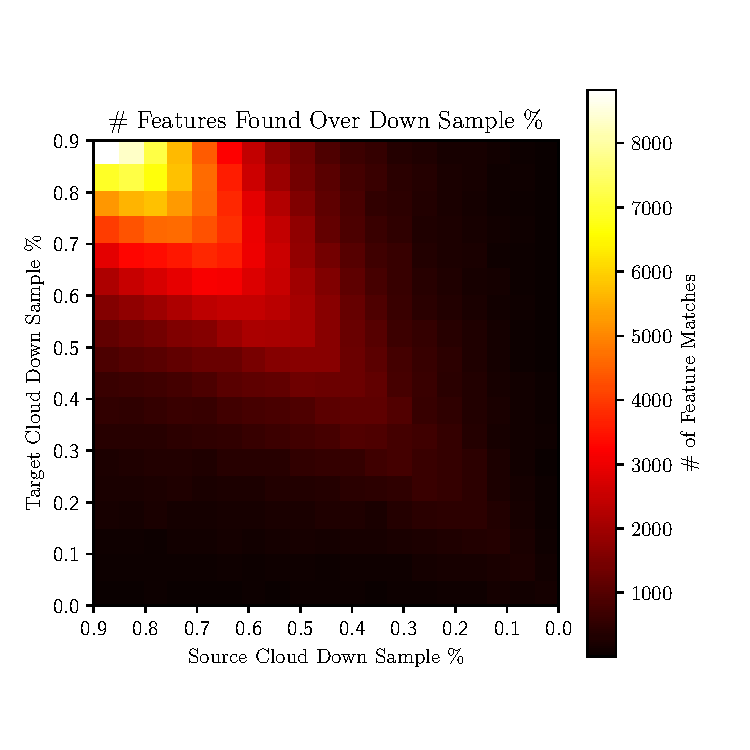
\includegraphics[width=\textwidth]{chapters/2-pose-estimation/fig/M.pdf}
		\caption{The source \gls{pc} generated from simulated contact points.\newline}
		\label{fig:pe-feature-filtered-pc}
	\end{subfigure}
	% \hfill
	\begin{subfigure}[b]{0.48\textwidth}
		\centering
		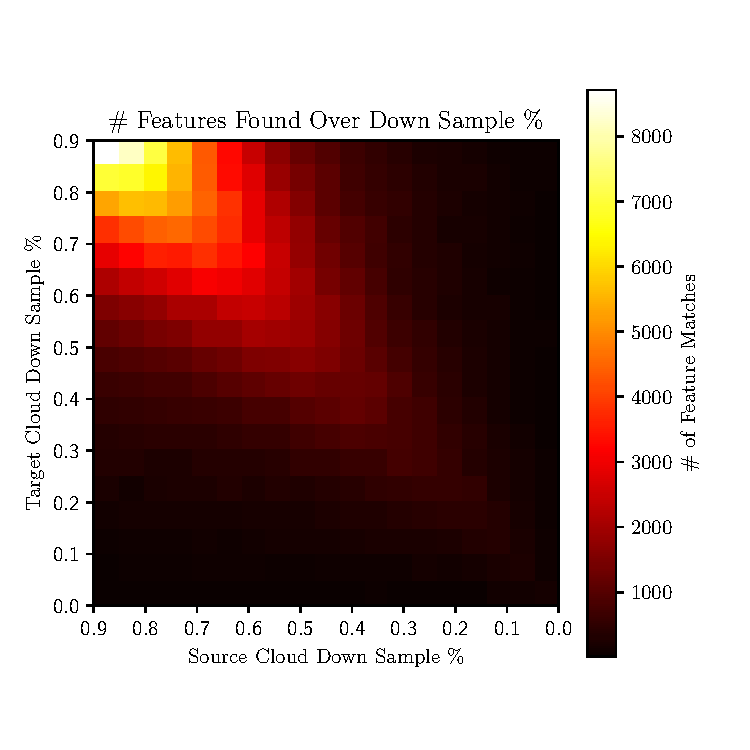
\includegraphics[width=\textwidth]{chapters/2-pose-estimation/fig/M_unfiltered.pdf}
		\caption{The target \gls{pc} generated by sampling the model mesh with \num{10,000} points.}
		\label{fig:pe-feature-unfiltered-pc}
	\end{subfigure}
	\caption{3D plots showing the sampled source and target \gls{pc}s along with a plot showing both of them overlaid.}
	\label{fig:pe-filture-and-unfiltered-pc}
\end{figure}


% In order to sample dat
% Here we cite the related work by \texttt{\textbackslash cite\{source-label\}} like this \cite{recent-progress-in-technologies-for-tactile-sensors}

\section{Results}\label{sec:2-pose-estimation-results}


\section{Discussion}\label{sec:2-pose-estimation-discussion}

\section{Conclusion}\label{sec:2-pose-estimation-conclusion}